\begin{frame}[fragile]{Issues in Word Representation}

  \begin{itemize}
    \item We cannot gain information of relation between words if those words in text is represented as one-hot encoding.
    \item The one-hot encoding would be very sparse if there exists large amount of unique words.
  \end{itemize}

  For example, we set hotel and motel as two different representative of one-hot encoding:

  \begin{center}
    motel = [0,0,0,0,1,0,0,0,0] \\
    hotel = [0,0,0,0,0,1,0,0,0]
  \end{center}

  We have no idea how motel and hotel are relate to each other while those two vectors are orthogonal! That's why we introduce word embedding approach to tackle these problems. \cite{word2vec}

\end{frame}

\begin{frame}[fragile]{Word Embedding}

  \begin{center}
    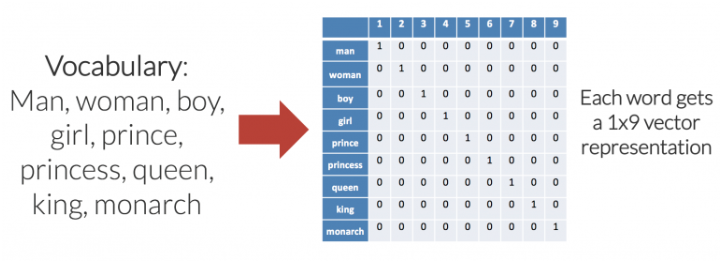
\includegraphics[scale=0.3]{../images/img_2.png} \\
    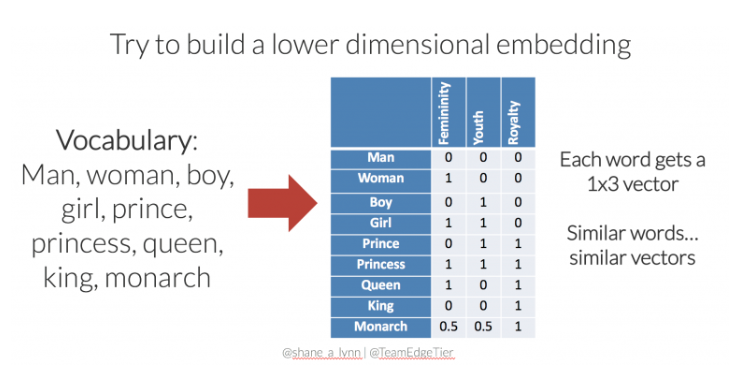
\includegraphics[scale=0.3]{../images/img_3.png} \\
    \href{https://www.shanelynn.ie/get-busy-with-word-embeddings-introduction/}{[Image Source]}
  \end{center}



\end{frame}

\begin{frame}[fragile]{Word2Vec}

  \begin{center}
    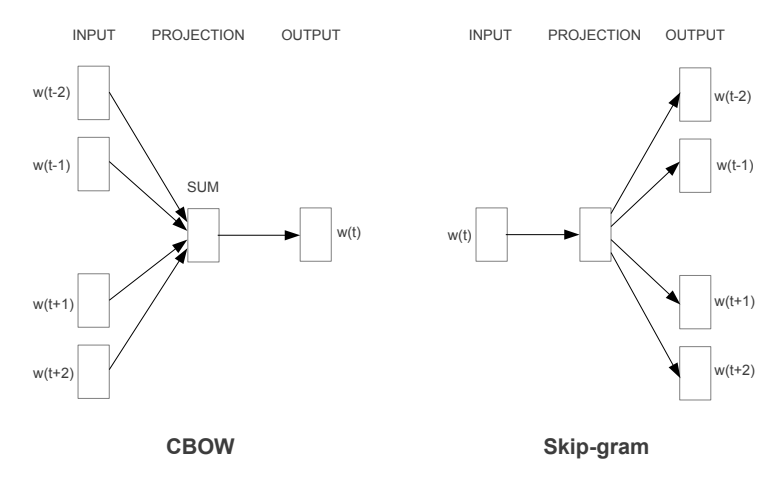
\includegraphics[scale=0.3]{../images/img_4.png}
  \end{center}

\end{frame}

\begin{frame}[fragile]{CBOW}

  \begin{center}
    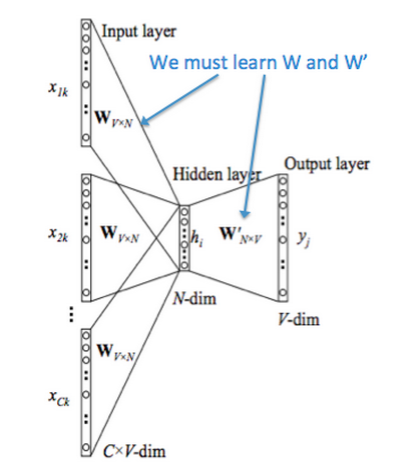
\includegraphics[scale=0.4]{../images/img_5.png} \\
    \href{https://web.stanford.edu/class/archive/cs/cs224n/cs224n.1214/readings/cs224n-2019-notes01-wordvecs1.pdf}{[Image Source]}
  \end{center}


  Use the probability $P(y_{i} | x_{1k}, x_{2k}, ... , x_{Ck})$ to learn the weight matrix $W$!
\end{frame}